%%
%% Beuth Hochschule für Technik --  
%%
%% Kapitel 3 - Desktop App
%%
%%	
\lstset{language=Java,
				backgroundcolor=\color{light-gray},
				%frame=single,
				tabsize=2,
				breaklines=true,
				%numbers=left,
				numbersep=5pt,
				%numberstyle=\color{light-gray},
				basicstyle=\ttfamily\color{black}\small,
				keywordstyle=\color{HKS51}\bfseries,
				commentstyle=\color{HKS13}\slshape,,
				identifierstyle=\color{blue},
				stringstyle =\color{orange}}
				
				
\chapter{Technische Umsetzung}
Im Folgenden wird auf die Vorgehensweise eingegangen, welche Technologien verwendet worden sind und wie der Login- und Registrierungsprozess ablaufen soll, sowie die Unterschiede zwischen der Desktop-Anwendung und der Android-Applikation.



\section{Struktur und Aufbau der App}
Es gibt insgesamt vier verschiedene View's in der Applikation.
\begin{itemize}
	\item Login
	\item Registrierung
	\item Control
	\item Bilderlog
\end{itemize}

Im Anhang \ref{A.android} und \ref{A.desktop} befinden sich Screenshots der Applikationen.\\

\subsection{Login}
Bei der Login-View kann sich der Nutzer mit seinem Benutzernamen und Passwort, was in der Datenbank hinterlegt ist, anmelden und somit zur Control-View gelangen. Ist einer der Felder nicht ausgefüllt oder das Passwort bzw. der User nicht korrekt, wird das mit einer Fehlermeldung dargestellt und der Nutzer kann es erneut versuchen. Das Passwort-Feld ist immer maskiert. Von der Login-View ist es auch möglich, zur Registrierung-View zu wechseln.\\


\begin{figure}[h]
  \begin{center}
    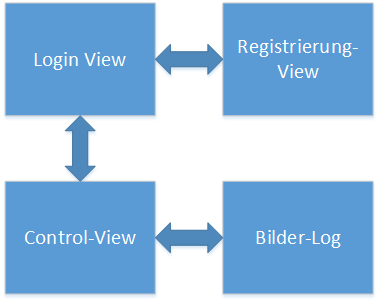
\includegraphics[scale=0.5]{Views.png}
  		  \caption{Wechseln zwischen Views}
     \label{fig.Views}
  \end{center}
\end{figure}


\subsection{Registrierung}
Falls der Benutzer noch kein Account in der Datenbanktabelle \texttt{tb\_users} hat, hat er die Möglichkeit, sich über die Registrierung-View zu registrieren. Software-seitig wurde eine Überprüfung eingebaut, dass jedes Textfeld etwas beinhalten muss (Pflichtfelder). Die Passwörter werden auf Konsistenz überprüft. Wenn alle Überprüfungen korrekt sind, wird aus den Eingaben ein String gebaut und an die Datenbank geschickt. Falls die Überprüfung fehlgeschlagen ist, wird wie bei der Login-View eine Fehlermeldung ausgegeben. An dieser Stelle wird auch überprüft, ob der Benutzername schon in der Datenbanktabelle \texttt{tb\_users} existiert. Somit wird Doppeleinträge in der Datenbanktabelle verhindert.\\

\subsection{Datenbankverbindung}
Bei der Datenbankverbindung ist zu beachten, dass die Desktop-Anwendung sich direkt mit dem MySQL-Server verbinden kann, die Android Applikation allerdings nicht, weil die entsprechenden MySQL-Bibliotheken für Android zu diesem Zeitpunkt nicht existieren. Die Verbindung findet über \texttt{JSON} statt. Server-seitig existiert ein \texttt{PHP}-Skript, welches das JSON-Objekt abfängt und die Verbindung zur Datenbank herstellt.\\

\subsubsection{JSON}

Es wird eine Liste \texttt{params} mit dem Typ \texttt{NameValuePair} erzeugt. Anschließend werden die Übergabeparameter in die Liste eingefügt mit der Methode \texttt{params.add()}, zusätzlich mit einem Tag \texttt{register\_tag}. Im Nachhinein wird das JSON-Objekt zusammengefügt und am Ende der Funktion das fertig erzeugte JSON-Objekt mit allen Inhalten zurückgegeben. Das erzeugte JSON-Objekt wird per POST-Methode an den Server gesendet. Auf dem Server wird in der \textit{insert.php} anhand des Tags erkannt, dass sich ein neuer Nutzer registrieren möchte. Das PHP-Skript baut eine Verbindung zur MySQL-Datenbank auf und sendet die Daten als SQL-Syntax dorthin und trägt diese in die jeweiligen Spalten ein. In der Login-View ist der Vorgang gleich, nur wird auf dem Server diesmal die \textit{login.php} angesprochen.\\

\begin{lstlisting}[caption={User Functions},captionpos=b]
    public JSONObject loginUser(String name, String password);
    public JSONObject registerUser(String name,  String password);
    public boolean isUserLoggedIn(Context context);
    public boolean logoutUser(Context context);
    
    // Building Parameters

   List<NameValuePair> params = new ArrayList<NameValuePair>();
   params.add(new BasicNameValuePair("tag", register_tag));
   params.add(new BasicNameValuePair("name", name));
   params.add(new BasicNameValuePair("password", password));

   // getting JSON Object
   JSONParser jsonParser = new JSONParser(registerURL, params,mContext);
   try {
         Thread.sleep(2000);
   } catch (InterruptedException e) {
         e.printStackTrace();
   }
   JSONObject json = jsonParser.getJSONFromUrl();
   Log.i("JSON4", json.toString());
   // return json
   return json;
\end{lstlisting}


\subsubsection{MySQL}
Bei der Desktop-Anwendung existiert eine Klasse namens \texttt{DBConnector.java}, die für die Verbindung zur Datenbank zuständig ist. Dank dieser Klasse und der direkten Verbindung kann die Anwendung SQL Befehle direkt an den Server schicken. Um ein Eintrag zu erstellen, bereitet die Applikation ein String vor, mit der SQL-Syntax und die Parameter die eingetragen werden sollen. Der folgende Code zeigt die Darstellung, wie ein String mit Nutzerdaten aussieht und an die Datenbank gesendet wird.


\begin{lstlisting}[caption={String neuer Benutzer}\label{lst:reg.java.eintrag},captionpos=b]
	String SQL = "INSERT INTO tb_user VALUES (null,'"
									+ txtVorname.getText() + "', '"
									+ txtNachname.getText() + "', '"
									+ txtEmail.getText() + "', '"
									+ txtUserName.getText() + "', '"
									+ txtPw.getText() + "', NOW())";
\end{lstlisting}

\begin{lstlisting}[caption={SQL Benutzer eintragen}
,captionpos=b]
	INSERT INTO tb_user VALUES (null,'Heinz', 'Müller', 'heinz.mueller@gmail.com', 'H.Mueller', '007', NOW())
\end{lstlisting}

Der Befehl \texttt{NOW()} wird in der Datenbank mit dem aktuellen Datum und Uhrzeit gesetzt.\\

\subsection{Control}
In der View \texttt{Control} ist es möglich, das Live-Video von der Kamera zu betrachten. Es wird mit Hilfe der Klasse \textit{WebEngine} und \textit{WebView} realisiert. D.h. es wird durch \textit{WebEngine} die Webseite geladen und durch \textit{WebView} wird die geladene Webseite in der View angezeigt. Diese Webseite wird vom \textit{MJPG Streamer} (siehe Kapitel \ref{mjpg}) zur Verfügung gestellt. Der Stream wird erst gestartet, wenn der Button \texttt{Stream starten} getätigt ist.

\newpage

\begin{lstlisting}[caption={Stream Einbindung},captionpos=b]
WebView webview = new WebView();
webview.setVisible(true);
WebEngine webengine = webview.getEngine();
webengine.setJavaScriptEnabled(true);
File file = new File("http://<IP-Adresse vom PI>/javascript\_simple.html");
webengine.load(file.toString());
\end{lstlisting}

Beim Betätigen des Buttons \textit{Bilderlog} wird eine neue View geöffnet (siehe Kapital \ref{bilderLog}) und die View \texttt{Control} wird geschlossen. Nach dem Betätigen des Buttons \texttt{Tür öffnen} werden zwei Funktionen aufgerufen. Bei der ersten Funktion wird über die Socket-Schnittstelle ein Befehl an das Pi gesendet, das dieses die Tür öffnen soll. Bei der zweiten Funktion wird ein neuer Eintrag in die Tabelle \texttt{tb\_doorloogers} in Datenbank eingetragen. Dieser Eintrag beinhaltet den Zeitpunkt des Öffnens der Tür, sowie der Benutzer. Der Server erstellt ein zweiter Eintrag, das bereits in Kapitel \ref{Socket} erläutert wurde.\\


\subsection{Bilder Log}\label{bilderLog}
Diese View hat als Hauptobjekt eine Tabelle (TableView). Der Tabelleninhalt wird dynamisch erstellt. In einer zusätzliche Klasse wird überprüft, wie viele Spalten die Datenbanktabelle hat und fügt diese dann dem Tabellen-Objekt hinzu. Nach dem Hinzufügen der Spalten wird Zeile für Zeile aus der Datenbank gelesen und in die Tabelle geladen. Zu jedem Eintrag in die Datenbanktabelle \texttt{tb\_doorlogger} gehört ein Bild. Um sich zu einen entsprechenden Tabelleneintrag das Bild anzusehen, kann der Benutzer ein Bild aus der dargestellten Tabelle auswählen.\\







%\section{Was ist JavaFX ?}

%
%
%
%In JavaFX ist ein Fenster ein Stage-Objekt. In diesem Stage-Objekt sind fünf verschiedenen View's implementiert. Diesen View-Objekte können mehrere anderer Objekte hinzugefügt werden. Bei diesen anderen Objekten kann es sich um Buttons, eine Tabelle, ein Textfeld usw. handeln.
%
%\begin{figure}[h]
%  \begin{center}
%    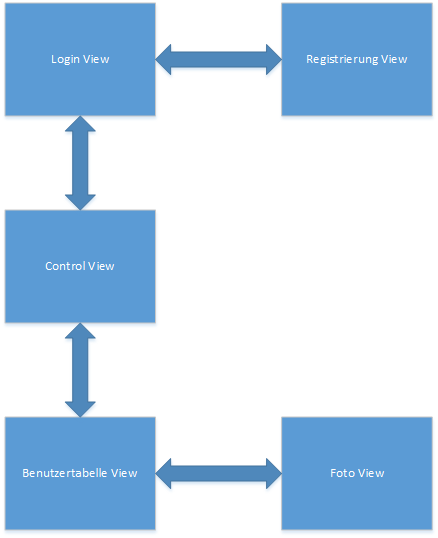
\includegraphics[scale=0.7]{MaskenDesktopVersion.png}
%  		  \caption{Aufbau der App}
%     \label{fig.MaskenDesktopVersion}
%  \end{center}
%\end{figure}\newpage
%
%\subsection{Login}
%\label{subsec.login}
%
%\begin{figure}[h]
%  \begin{center}
%    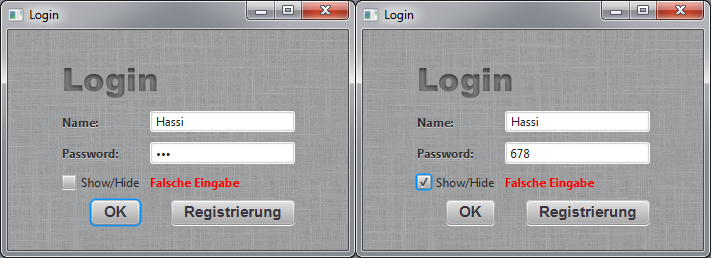
\includegraphics[scale=0.6]{loginStage.png}
%  		  \caption{Login View}
%     \label{fig.loginFenster}
%  \end{center}
%\end{figure}
%
%\subsection{Registrierung}
%\label{subsec.registrierung}

%%%%%%%%%%%%%%%%%%%%%%%%%%%%%%%%%%%%%%%%%%%%%%%%%%%%%%%%%%%%%%%%%%%%%%%%%%%
%referenz auf die DB wie sie aufgebaut ist ???
%%%%%%%%%%%%%%%%%%%%%%%%%%%%%%%%%%%%%%%%%%%%%%%%%%%%%%%%%%%%%%%%%%%%%%%%%%%

%
%Der Befehl \texttt{NOW()} wird in der Datenbank mit dem aktuellen Datum und Uhrzeit gesetzt.
%Die Sichtbarkeit der Anmeldedaten ist nur direkt innerhalb der Applikation möglich. In diesem Fall mit einem System.out.println() in Eclipse. Was noch  implementiert wurde, ist eine zusätzliche Freischaltung des neuen Users von einem Administrator. Nach direkter Registrierung und Freischaltung von einem Administrator kann sich der User anmelden.
%\begin{figure}[h]
%  \begin{center}
%    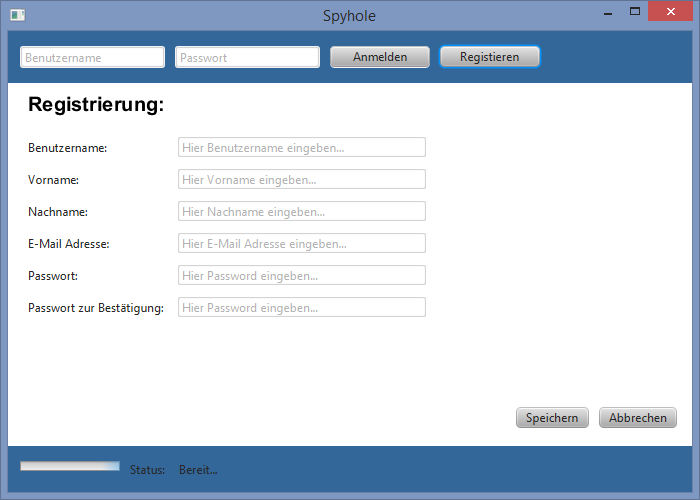
\includegraphics[scale=0.6]{regStage.png}
%  		  \caption{Registrierung View}
%     \label{fig.RegistrierungFenster}
%  \end{center}
%\end{figure}

%\subsection{Control}
%\label{subsec.control}

%In der View \texttt{Control} ist es möglich, das Live-Video von der Cam zu betrachten. Es wird mit Hilfe der Klasse WebEngine und WebView realisiert. D.h. es wird durch WebEngine die Webseite geladen und durch WebView wird die geladene Webseite in View angezeigt. Diese Webseite wird vom MJPEG Streamer zur Verfügung gestellt. Der Stream wird erst gestartet, wenn der Button \texttt{Stream starten} getätigt ist.
%
%\begin{lstlisting}[caption={Stream Einbindung}\label{lst:reg.java.stream},captionpos=b]
%WebView webview = new WebView();
%webview.setVisible(true);
%WebEngine webengine = webview.getEngine();
%webengine.setJavaScriptEnabled(true);
%File file = new File("http://<IP-Adresse vom PI>/javascript\_simple.html");
%webengine.load(file.toString());
%\end{lstlisting}
%
%Beim Betätigen des Buttons \texttt{Benutzertabelle} wird eine neue View \texttt{Datenbank} geöffnet (siehe Kapital \ref{subsec.datenbank}) und die View \texttt{Control} wird geschlossen. 
%Nach dem Betätigen des Buttons \texttt{Tür öffnen} werden zwei Funktionen aufgerufen. Bei der ersten Funktion wird über die Socket-Schnittstelle ein Befehl an das Pi gesendet, das dieses die Tür öffnen kann. Bei der zweiten Funktion wird ein neuer Eintrag in die Tabelle \texttt{tb\_doorloogers} in Datenbank eingetragen. Dieser Eintrag beinhaltet den Zeitpunkt des Öffnens der Tür.



%\subsection{Datenbank}
%\label{subsec.datenbank}
%Diese View hat als Hauptobjekt eine Tabelle (TableView). Der Tabelleninhalt wird dynamisch erstellt. In einer zusätzliche Klasse wird überprüft, wie viele Spalten die Datenbank hat und fügt diese dann dem Tabellen-Objekt hinzu. Nach dem Hinzufügen der Spalten wird Zeile für Zeile aus der Datenbank geladen und in die Tabelle gefüllt. Zu jedem Eintrag in die Datenbanktabelle \texttt{tb\_doorlogger} gehört ein Bild. Um sich zu einen entsprechenden Tabelleneintrag das Bild anzusehen, muss man über eine Combobox die ID der Zeile auswählen und auf den Button \texttt{Bild laden} klicken. Im Moment ist die Implementierung der TableView noch nicht fertig, daher funktioniert die TableView mit Darstellung der Bilder nicht richtig. %Mehr dazu im Kapitel \ref{subsec.foto}. %Die Combobox zeigt nur so viele Zahlen wie es Zeilen in der Tabelle gibt. Wenn nichts in der Datenbank steht und dadurch auch kein Eintrag in die Tabelle gemacht wird, werden die Combobox und der \texttt{Open Picture} Button deaktiviert. Gibt es Einträge in der Datenbank, so ist die Standarteinstellung der Combobox auf 1.



%\subsection{Foto}
%\label{subsec.foto}
%Nachdem der \texttt{Bild laden} Button in der Datenbank Ansicht gedrückt wurde, wird mit Hilfe der angegebenen ID aus der Combobox der SQL-String gebaut.
%
%\begin{lstlisting}[caption={Java-SQL String Foto öffnen}\label{lst:pic.db.foto.open},captionpos=b]
%String SQL = "SELECT * FROM tb_images WHERE ID = " + userID;
%\end{lstlisting}
%
%Aus dem String ist relativ leicht zu erkennen, dass das Bild aus der Datenbanktabelle \texttt{tb\_images} kommt. Das Bild ist aber in der Datenbank nur binär als BLOB Typ abgelegt. Dieser Typ existiert auch in Java. Nach dem Auslesen des Binärstreams wandeln wir das Gelesene in ein Byte-Array. Aus dem Byte-Array erzeugen wir dann ein Buffered-Image. In Swing könnten wir uns jetzt schon ein Bild anzeigen lassen. Aber die App wurde ja nicht mit Swing, sondern mit JavaFX geschrieben. Dank eines \texttt{.toFXImage(BufferedImage arg0, WritableImage arg1)} Befehles lässt sich unser Swing-Objekt einfach in ein JavaFX-Objekt umwandeln. Da im Moment die Benutzertabelle View noch nicht fertig implementiert ist, zeigen wir dieses Objekt vorrübergehend in einem zusätzlichen Stage Fenster an. In der Zukunft sollen die Bilder nicht in einem zusätzlichen Fenster dargestellt werden, sondern in einer zusätzlichen View-Objekt in Benutzertabelle View. %Ein klarer Vorteil bei dieser Methode ist, dass es nicht wichtig ist, was für ein Typ dem Bild mal angehörte.\newpage
%\begin{lstlisting}[caption={JavaFX Foto öffnen}\label{lst:pic.javafx.open},captionpos=b]
%//Foto aus DB holen
%byte[] imgData = imgShow.getImageDB(userID);
%...
%//Foto nach JavaFX Objekt wandeln
%SwingFXUtils.toFXImage(bufImg, img2);
%
%//Foto imageView hinzufügen
%imageView.setImage(img2);
%\end{lstlisting}

%\section{Problematik der Verwaltung der Fenster}
%Während der Entwicklung der Desktop Applikation in JavaFX gab es technische Schwierigkeiten mit der Schließung der einzelnen Fenster. Wenn im Fenster ein Button betätigt wird, der gleichzeitig ein neues Fenster öffnen und das aktuelle Fenster schließen soll, wird ungewollt der gesamte Java-Applikation Prozess gekillt. Besonders bei dem Fenster mit dem Stream gab es ein weiteres Problem, dass nach der Schließung des Stream-Fensters der Stream im Hintergrund weiterlief. Es muss ein Konzept zur korrekten Schließung der Fenster erstellt werden, sodass eine Window-Klasse die einzelnen Fenster zur Öffnung und Schließung steuert. Das Konzept wurde zum Teil aus Zeitgründen nicht vollständig umgesetzt. Die Umsetzung wurde jetzt so realisiert, dass das aktuelle Fenster zuerst das kommende Fenster aufruft, dann wird erst das aktuelle Fenster geschlossen. Bei dem Fenster mit dem Stream wurde nicht mit der Klasse \texttt{MediaView} sowie \texttt{MediaPlayer} gearbeitet, sondern mit der Klasse \texttt{webView} und \texttt{webEngine}. Damit konnte auch das Problem mit dem ungewollten Weiterlaufen des Streams im Hintergrund gelöst werden.